\documentclass{beamer}

\mode<presentation>{
\usetheme{Madrid}
}

\setbeamertemplate{footline}[page number]

\usepackage[utf8]{inputenc}
\usepackage[ngerman]{babel}
\usepackage{graphicx}
\usepackage{multirow}
\usepackage{array}
\usepackage{colortbl}	

\usepackage{xcolor}
\usepackage{tikz} %Zeichnungen

\definecolor{darkblue}{rgb}{0, 0, 0.4}
\definecolor{cornellred}{rgb}{0.7, 0.11, 0.11}

\title[Rüchardt-Methode]{Adiabatenkoeffizient}
\author{Marius Ising}
\institute{Grundpraktikum Physik Teil I}
%\date{\today}


\begin{document}

%Titelseite
\begin{frame}
\titlepage
\end{frame}

%Inhaltsverzeichnis
\begin{frame}
\frametitle{Inhalt}
\tableofcontents
\end{frame}


\section{Rüchardt-Methode}

\begin{frame}
\frametitle{Rüchardt-Methode}

\begin{columns}[c]
\column{.7\textwidth}
\begin{block}{Bewegungsgleichung (Gedämpfte Schwingung)}
$$\frac{d^2x}{dt^2} + \frac{\alpha}m \frac{dx}{dt} + \frac{p\kappa A^2}{mV}x = 0$$
\end{block}

Lösung: \hspace{0.2cm} $x(t) = e^{-\delta t}\cos(\omega t+\varphi)$ \hspace{0.2cm} mit \hspace{0.2cm} $\delta = \frac{\alpha}{2m}$. \\
$$\omega_0^2 = \frac{p\kappa A^2}{mV} = \omega^2 + \delta^2$$


\begin{block}{Adiabatenkoeffizient}
$$\kappa = \frac{mV}{pA^2}\omega_0^2$$
\end{block}


\column{0.25\textwidth}
\begin{tikzpicture}[scale=0.45]
\draw (0,0) -- (0,1) -- (-0.2,1) -- (-0.2,1.2) -- (1.2,1.2) -- (1.2,1) -- (1,1) -- (1,0) -- (3.5,-6) -- (-2.5,-6) -- (0,0);
\draw (0.15,0) -- (0.15,10) -- (0.85,10) -- (0.85,0) -- (0.15,0); 
\fill[cornellred] (0,0.75) rectangle (1,1.4); 
\fill[darkblue] (0.5,6.5) circle(0.35);
\node at (0.5,-4.5) {$pV^\kappa = const$};
\draw[->] (0.5,7) -- (0.5,8);
\draw[->] (0.5,6) -- (0.5,5);
\end{tikzpicture}

\end{columns}
\end{frame}


\section{Versuchsaufbau}

\begin{frame}
\frametitle{Versuchsaufbau}
\begin{figure}
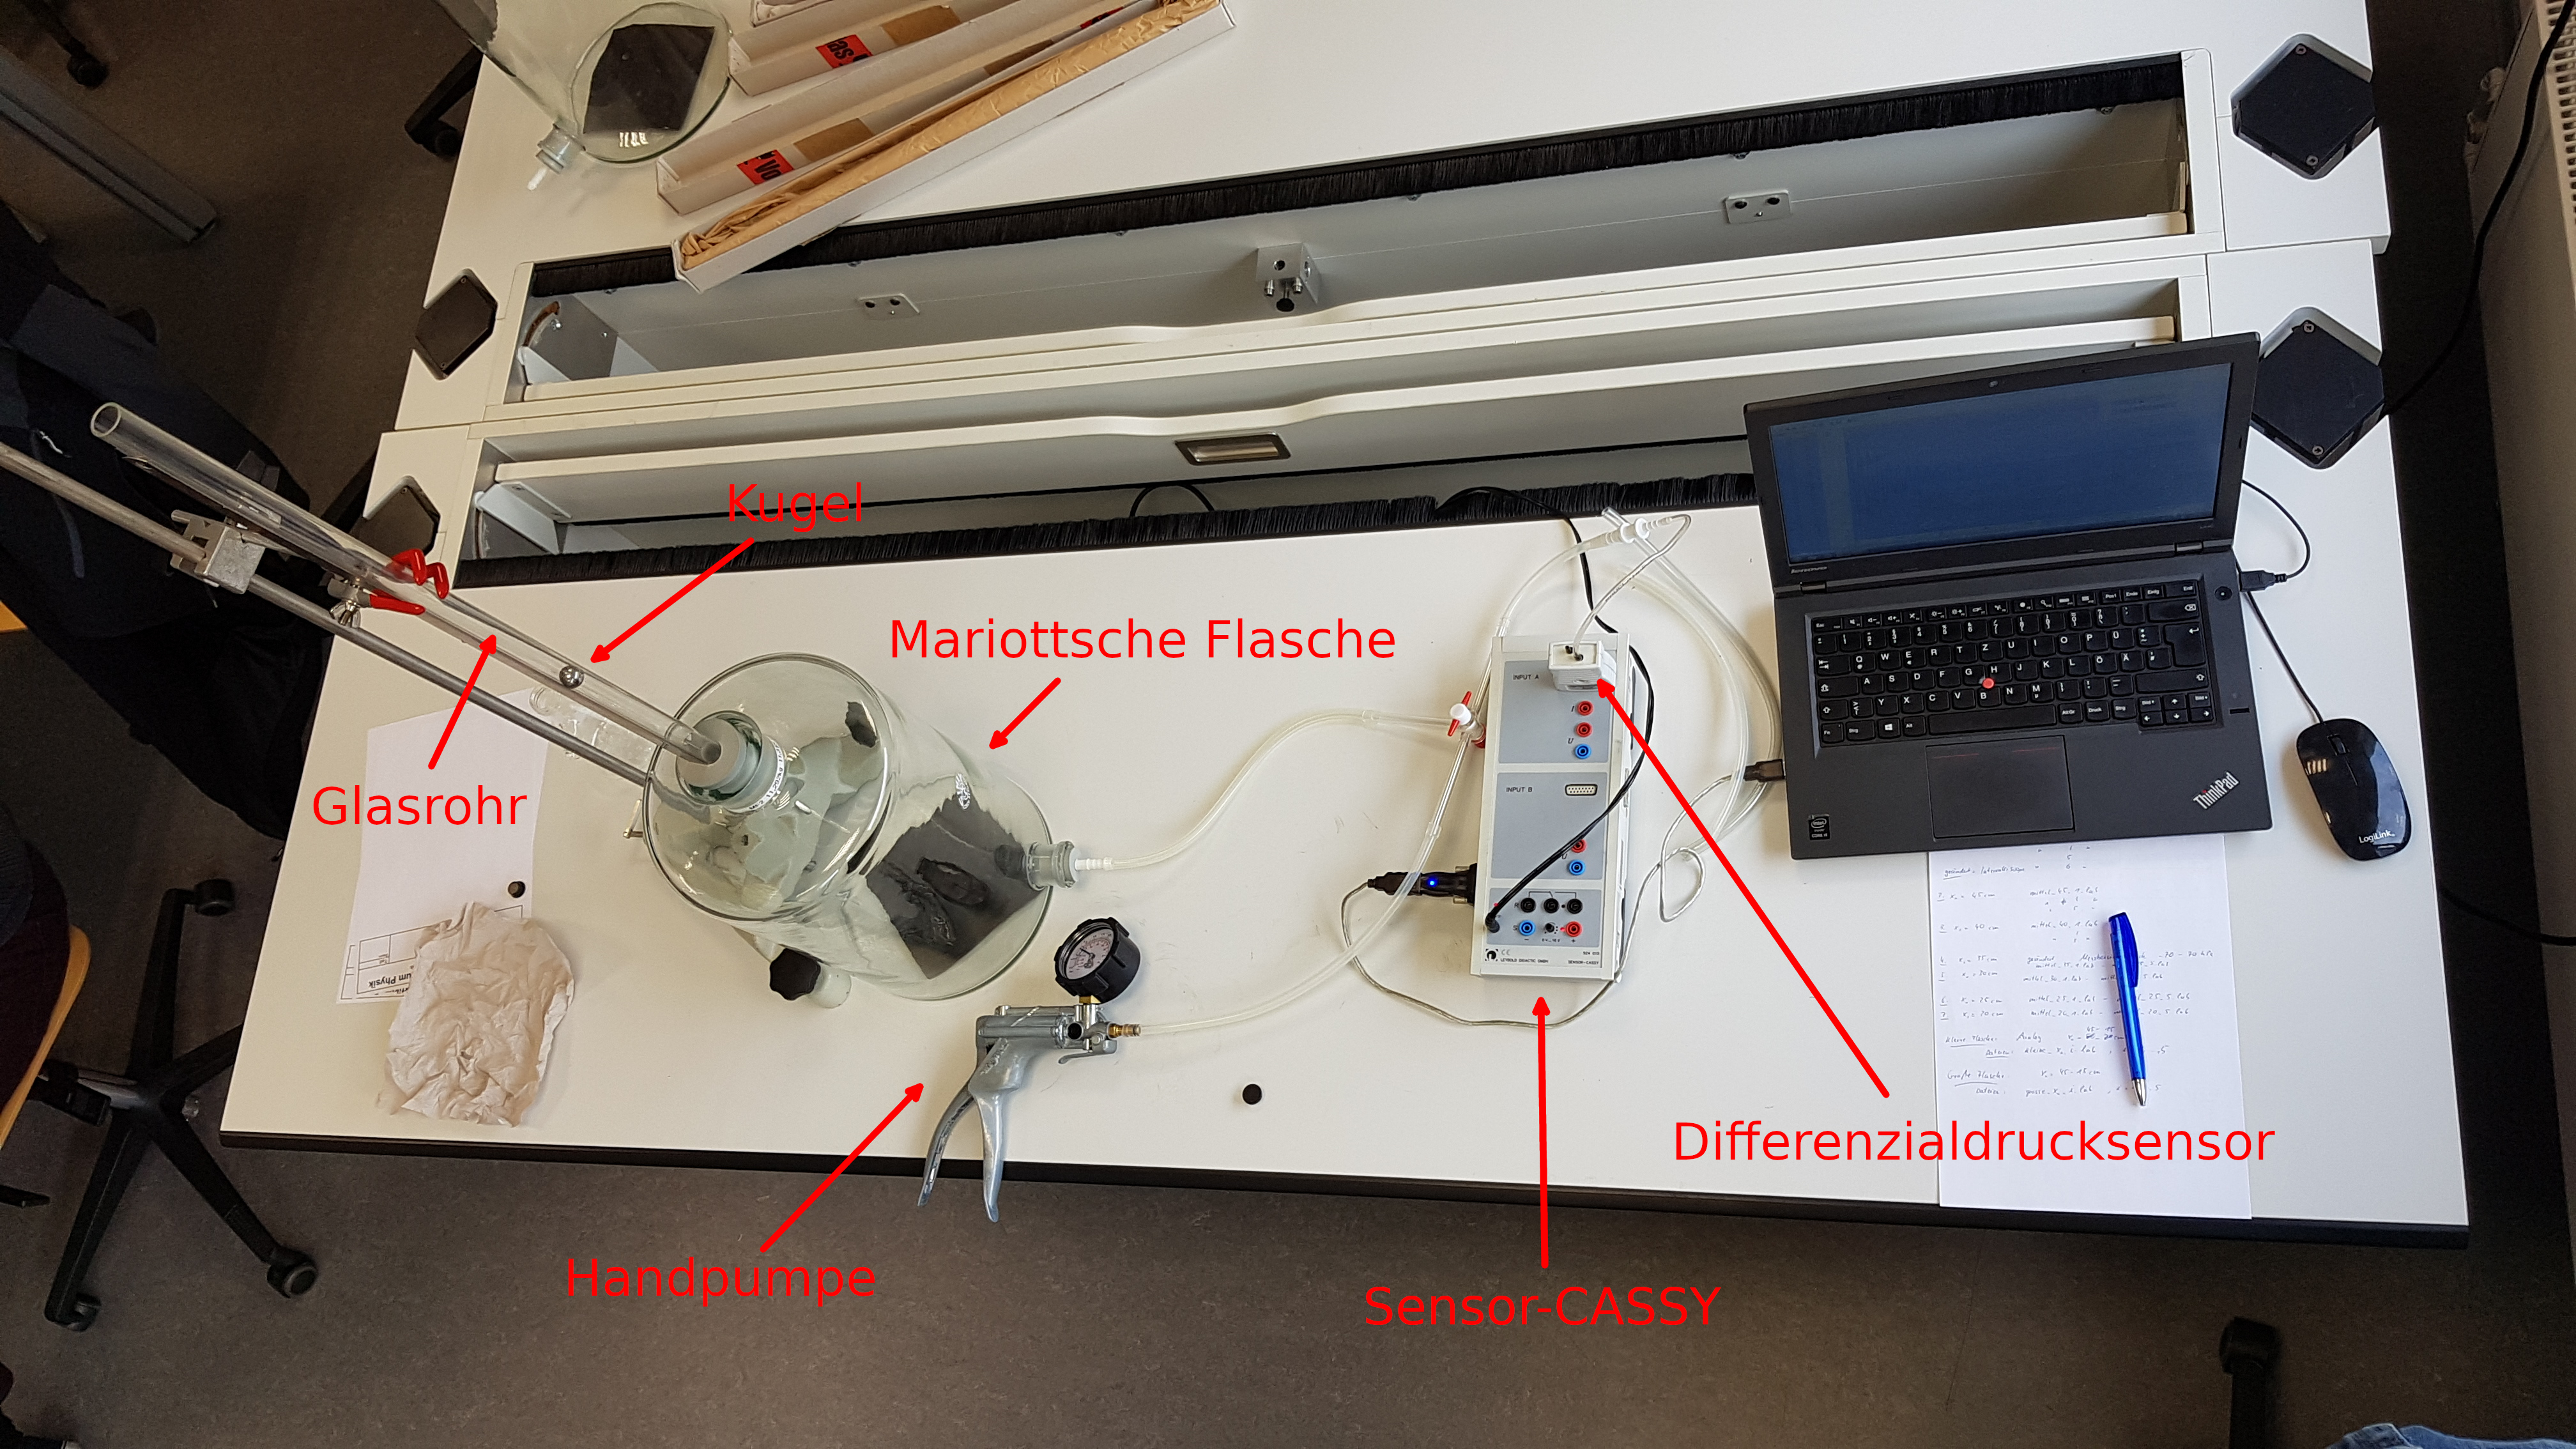
\includegraphics[width=\linewidth]{bilder/aufbau_beschriftet.jpg}
\end{figure}
\end{frame}


\section{Versuchsdurchführung}

\begin{frame}
\frametitle{Versuchsdurchführung}

\begin{enumerate}[-]
\item 3 Flaschen unterschiedlicher Größe
\item 6-7 Starthöhen pro Flasche
\item 5 Messungen pro Starthöhe
\item Messbereich: $\pm$ 21 hPa oder $\pm$ 70 hPa
\end{enumerate}

\begin{table}
\begin{tabular}{|c|c|c|c|c|}
\hline
\multirow{2}{*}{Anzahl} & \multicolumn{2}{c|}{Messintervall} & \multicolumn{2}{c|}{Messzeit} \\
\cline{2-5}
& Gruppe 1 & Gruppe 2 & Gruppe 1 & Gruppe 2 \\
\hline
16000 & 1 ms & 200-500 $\mu$s & 16 s & 3.2-8 s \\
\hline
\end{tabular}
\caption{Messparameter}
\end{table}
\end{frame}

\section{Versuchsauswertung}

\begin{frame}
\frametitle{Versuchsauswertung}
\begin{figure}
\includegraphics[width=.9\linewidth]{plots/rohdaten_log.pdf}
\end{figure}
\end{frame}

\subsection{Frequenzbestimmung}

\begin{frame}
\frametitle{Frequenzbestimmung}

\begin{figure}
\centering
\includegraphics[width=0.8\textwidth]{plots/FFT.jpg}
\caption{FFT mit Peakfinder und Fehler}
\end{figure}

\end{frame}

\subsection{Dämpfungsbestimmung}

\begin{frame}
\frametitle{Dämpfungsbestimmung}

Modell: \hspace{0.2cm} $p(t) = Ae^{-\delta t} \sin(\omega t + \varphi) + B$

\begin{enumerate}[-]
\item Schätzung von $B$ nach dem Abklingen
\item Ablesen zweier Maxima (0.0029-0.029 hPa Ablesefehler)
\item $\delta = f\ln\left( \frac{p(t_0)-B}{p(t_1)-B} \right)$
\end{enumerate}

\begin{figure}
\centering
\includegraphics[width=0.9\textwidth]{plots/anpassung_delta.pdf}
\end{figure}

\end{frame}


\subsection{Volumenbestimmung}

\begin{frame}
\frametitle{Volumenbestimmung}

\begin{block}{Volumen}
$$V = V_F + x_0A + V_r$$
\end{block}

\begin{table}
\begin{tabular}{|c|c|c|c|}
\hline
\multirow{2}{*}{Flasche} & \multicolumn{2}{c|}{Volumen $V_F$ / $10^{-6}\mathrm m^3$} & \multirow{2}{*}{Fehler $\sigma$ / $10^{-6}\mathrm m^3$} \\
\cline{2-3}
& Gruppe 1 & Gruppe 2 & \\
\hline
 kleine & 307.8 & 309.7 & 1\\
\hline
mittlere & 1139.6 & 1119.1 & 1\\
\hline
große & 11267 & 11315 & 50\\
\hline
\end{tabular}
\end{table}

\begin{block}{Lineare Regression}
$$(V_F+x_0A)\left( \frac 1{\omega_0^2} \right) = \frac{p\kappa A^2}m \frac 1{\omega_0^2} - V_r$$
\end{block}

\end{frame}


\begin{frame}
\frametitle{Volumenbestimmung}

\begin{figure}
\begin{minipage}[t]{0.49\linewidth}
\centering
\includegraphics[width=\linewidth]{plots/modell_2.jpg}
\end{minipage}
\hfill
\begin{minipage}[t]{0.49\linewidth}
\centering
\includegraphics[width=\linewidth]{plots/regression_2.jpg}
\end{minipage}
\end{figure}
Aus der Steigung: \hspace{0.2cm} $\kappa = 1.308 \pm 0.039$

\end{frame}


\begin{frame}
\frametitle{Volumenbestimmung}

\begin{figure}
\centering
\includegraphics[width=0.9\linewidth]{plots/regression_kleine.pdf}
\end{figure}

\begin{table}
\begin{tabular}{|c|c|c|}
\hline
Steigung $a$ / $\frac{\mathrm m^3}{\mathrm s^2}$ & $V_r$ / $\mathrm m^3$ & $\frac{\chi^2}{n_{df}}$ \\
\hline
$0.304 \pm 0.012$ & $(-7.9 \pm 14.5) \cdot 10^{-6}$ & 0.88 \\
\hline
\end{tabular}
\end{table}

\end{frame}


\begin{frame}
\frametitle{Versuchsauswertung}

\begin{table}
\begin{tabular}{|c|c|c|}
\hline
Größe & Wert & Fehler $\sigma$ \\
\hline
Masse $m$ & 16.5 g & 0.03 g \\
\hline
Höhe $x_0$ & 0.15 bis 0.5 m & 0.003 m \\
\hline
Durchmesser $d$ & 16.00 mm & 0.003 mm \\
\hline
Außendruck $p_0$ & 994 hPa & 0.3 hPa \\
\hline
\end{tabular}
\caption{Restliche Größen mit Fehlern}
\end{table}
Bestimmung des Adiabatenkoeffizienten mittels
$$\kappa = \omega_0^2\frac{mV}{pA^2} = (\delta^2 + 4\pi^2 f^2) \frac{(V_F+x_0\frac{\pi}4 d^2 + V_r)}{(p_0+\frac{4mg}{\pi d^2})\frac{\pi^2d^4}{16}}$$
und Gaußscher Fehlerfortplfanzung.
\end{frame}




\begin{frame}
\frametitle{Versuchsauswertung}

Aus theoretischer Überlegung: \hspace{0.2cm} $\kappa_L = \frac 75 = 1.4$

\begin{table}
\begin{tabular}{|c|c|c|c|c|}
\hline
\multirow{2}{*}{Flasche} & \multicolumn{2}{c|}{$\kappa$} & \multicolumn{2}{c|}{$\frac{|\kappa-\kappa_L|}\sigma$} \\
\cline{2-5}
& Gruppe 1 & Gruppe 2 & Gruppe 1 & Gruppe 2 \\
\hline
\multirow{2}{*}{kleine} & $1.307 \pm 1.043$ & $1.266 \pm 0.019$ & \cellcolor[rgb]{0.06,1,0} 0.09 & 
\cellcolor[rgb]{1,0,0} 7.05 \\
\cline{2-5}
& $1.308 \pm 0.039$ & & \cellcolor[rgb]{1,0.48,0} 2.36 & \\
\hline
mittlere & $1.320 \pm 0.342$ & $1.337 \pm 0.007$ & \cellcolor[rgb]{0.16,1,0} 0.23 & \cellcolor[rgb]{1,0,0} 9.00 \\
\hline
große & $1.354 \pm 0.039$ & $1.494 \pm 0.003$ & \cellcolor[rgb]{0.79,1,0} 1.18 & \cellcolor[rgb]{1,0,0} 31.3 \\
\hline
\end{tabular}
\caption{Ergebnisse}
\end{table}

Mit gewichtetem Mittel und äußerem Fehler
\begin{table}
\begin{tabular}{|c|c|}
\hline
$\bar\kappa$ & $\frac{|\kappa-\kappa_L|}\sigma$ \\
\hline
$1.464 \pm 0.029$ & 2.21 \\
\hline
\end{tabular}
\end{table}


\end{frame}



\section{Fazit}

\begin{frame}
\frametitle{Fazit}

\begin{enumerate}[-]
\item Schlechte Ergebnisse mit großen Fehlern oder sehr großen Abweichungen von der Theorie
\item Schwierige Bestimmung von $V$ mittels Regression
\end{enumerate}
\end{frame}

\end{document}
